



\begin{frame}{Introduction}
 \vspace*{-0.5cm}
 \begin{center}
  \includegraphics[width=0.95\textwidth]{figures/40-years-processor-trend}
 \end{center}
 {\tiny https://www.karlrupp.net/2015/06/40-years-of-microprocessor-trend-data/ }
\end{frame}

\begin{frame}{Introduction}
 \vspace*{-0.5cm}
 \begin{center}
  Theoretical Peak Performance \\
  \includegraphics[width=0.95\textwidth]{figures/gflops-dp}
 \end{center}
 \vspace*{-0.5cm}
 {\tiny https://www.karlrupp.net/2013/06/cpu-gpu-and-mic-hardware-characteristics-over-time/ }
\end{frame}

\begin{frame}{Introduction}
 \vspace*{-0.5cm}
 \begin{center}
  Theoretical Peak Performance per Watt \\
  \includegraphics[width=0.95\textwidth]{figures/gflops-per-watt-dp}
 \end{center}
 \vspace*{-0.5cm}
 {\tiny https://www.karlrupp.net/2013/06/cpu-gpu-and-mic-hardware-characteristics-over-time/ }
\end{frame}

\begin{frame}{Introduction}
 \vspace*{-0.5cm}
 \begin{center}
  Memory Bandwidth \\
  \includegraphics[width=0.95\textwidth]{figures/mem-bw}
 \end{center}
 \vspace*{-0.5cm}
 {\tiny https://www.karlrupp.net/2013/06/cpu-gpu-and-mic-hardware-characteristics-over-time/ }
\end{frame}

\begin{frame}{Introduction}
 \vspace*{-0.5cm}
 \begin{center}
  Theoretical Peak Performance (FLOPs) per Byte of Memory Bandwidth \\
  \includegraphics[width=0.95\textwidth]{figures/flop-per-byte-dp}
 \end{center}
 \vspace*{-0.5cm}
 {\tiny https://www.karlrupp.net/2013/06/cpu-gpu-and-mic-hardware-characteristics-over-time/ }
\end{frame}



\begin{frame}[fragile]{FLOPs and Bandwidth}

\  \begin{block}{Typical PETSc Operations}
  \begin{itemize}
   \item Vector operations (add, dot, etc.)
   \item Sparse matrix-vector products (Krylov solvers, smoothers, residuals, etc.)
  \end{itemize}
 \end{block}

 \begin{block}{Maximizing Memory Bandwidth}
  \begin{itemize}
   \item Read contiguous blocks of memory (contiguous access)
   \item Avoid unordered reads whenever possible
  \end{itemize}
 \end{block}

\end{frame}


\begin{frame}[fragile]{FLOPs and Bandwidth}

  \begin{block}{Check Memory Bandwidth Yourself}
  \begin{itemize}
   \item \lstinline|make streams|
   %\pause
   \item Performance question to \verb|petsc-maint|, about 2h ago:
   \begin{lstlisting}
np  speedup
1   1.0
2   1.85
3   2.25
4   2.37
(...)
39  2.47
40  2.45
Estimation of possible speedup of MPI programs based on Streams benchmark.
It appears you have 1 node(s)
    \end{lstlisting}
  \end{itemize}
 \end{block}

\end{frame}

\begin{frame}[fragile]{FLOPs and Bandwidth}

\begin{block}{How does Memory Bandwidth Scale with Cores?}
 \begin{itemize}
  \item Usually saturates quickly
  \item 8-16 processes/threads usually suffice
 \end{itemize}
\end{block}

\begin{center}
 \includegraphics[width=0.7\textwidth]{figures/stream}
\end{center}

\end{frame}



\begin{frame}[fragile]{FLOPs and Bandwidth}

\begin{block}{Offset Memory Access}
  \begin{lstlisting}
void work(double *x, double *y, double *z, int N, int k)
{
  for (size_t i=0; i<N; ++i)
    z[i+k] = x[i+k] + y[i+k];
}  
  \end{lstlisting}
\end{block}

\vspace*{-0.5cm}
\begin{center}
 \includegraphics[width=0.6\textwidth]{figures/offset}
\end{center}

\end{frame}




\begin{frame}[fragile]{FLOPs and Bandwidth}

\begin{block}{Strided Memory Access}
  \begin{lstlisting}
void work(double *x, double *y, double *z, int N, int k)
{
  for (size_t i=0; i<N; ++i)
    z[i*k] = x[i*k] + y[i*k];
}  
  \end{lstlisting}
\end{block}

\vspace*{-0.5cm}
\begin{center}
 \includegraphics[width=0.6\textwidth]{figures/strided-access}
\end{center}

\end{frame}


%%

\begin{frame}[fragile]{FLOPs and Bandwidth}

\begin{block}{Strided Memory Access}
  \begin{itemize}
   \item Array of structs problematic
  \end{itemize}
  \begin{lstlisting}  
typedef struct particle
{
  double pos_x; double pos_y; double pos_z;
  double vel_x; double vel_y; double vel_z;
  double mass;
} Particle;
  
void increase_mass(Particle *particles, int N)
{
  for (int i=0; i<N; ++i)
    particles[i].mass *= 2.0;
}  
  \end{lstlisting}
\end{block}
   %\pause
   \begin{center} 
\includegraphics[width=0.7\textwidth]{figures/particles-strided} \end{center}

\end{frame}

%%%

\begin{frame}[fragile]{FLOPs and Bandwidth}

\begin{block}{Strided Memory Access}
  \begin{itemize}
   \item Workaround: Structure of Arrays
  \end{itemize}
  \begin{lstlisting}  
typedef struct particles
{
  double *pos_x; double *pos_y; double *pos_z;
  double *vel_x; double *vel_y; double *vel_z;
  double *mass;
} Particle;
  
void increase_mass(Particle *particles, int N)
{
  for (int i=0; i<N; ++i)
    particles.mass[i] *= 2.0;
}  
  \end{lstlisting}
\end{block}

   %\pause
   \begin{center} \includegraphics[width=0.7\textwidth]{figures/particles-contiguous} \end{center} \vspace*{0.5cm}

\end{frame}


\begin{frame}{PETSc}
   \begin{center} \Large \textbf{Mindlessly applying object-oriented programming \\[1em]
                                 all the way down to fine granularity \\[1em]
                                 is a recipe for a performance disaster.} \end{center}
                                                                               
\end{frame}
